\documentclass[border=10pt]{standalone}

\usepackage{tikz}
\usepackage{tikzsymbols}
\usetikzlibrary{calc,patterns,shapes.geometric}

\def\centerarc[#1](#2)(#3:#4:#5){\draw[#1] ($(#2)+({#5*cos(#3)},{#5*sin(#3)})$) arc (#3:#4:#5);}

\begin{document}
	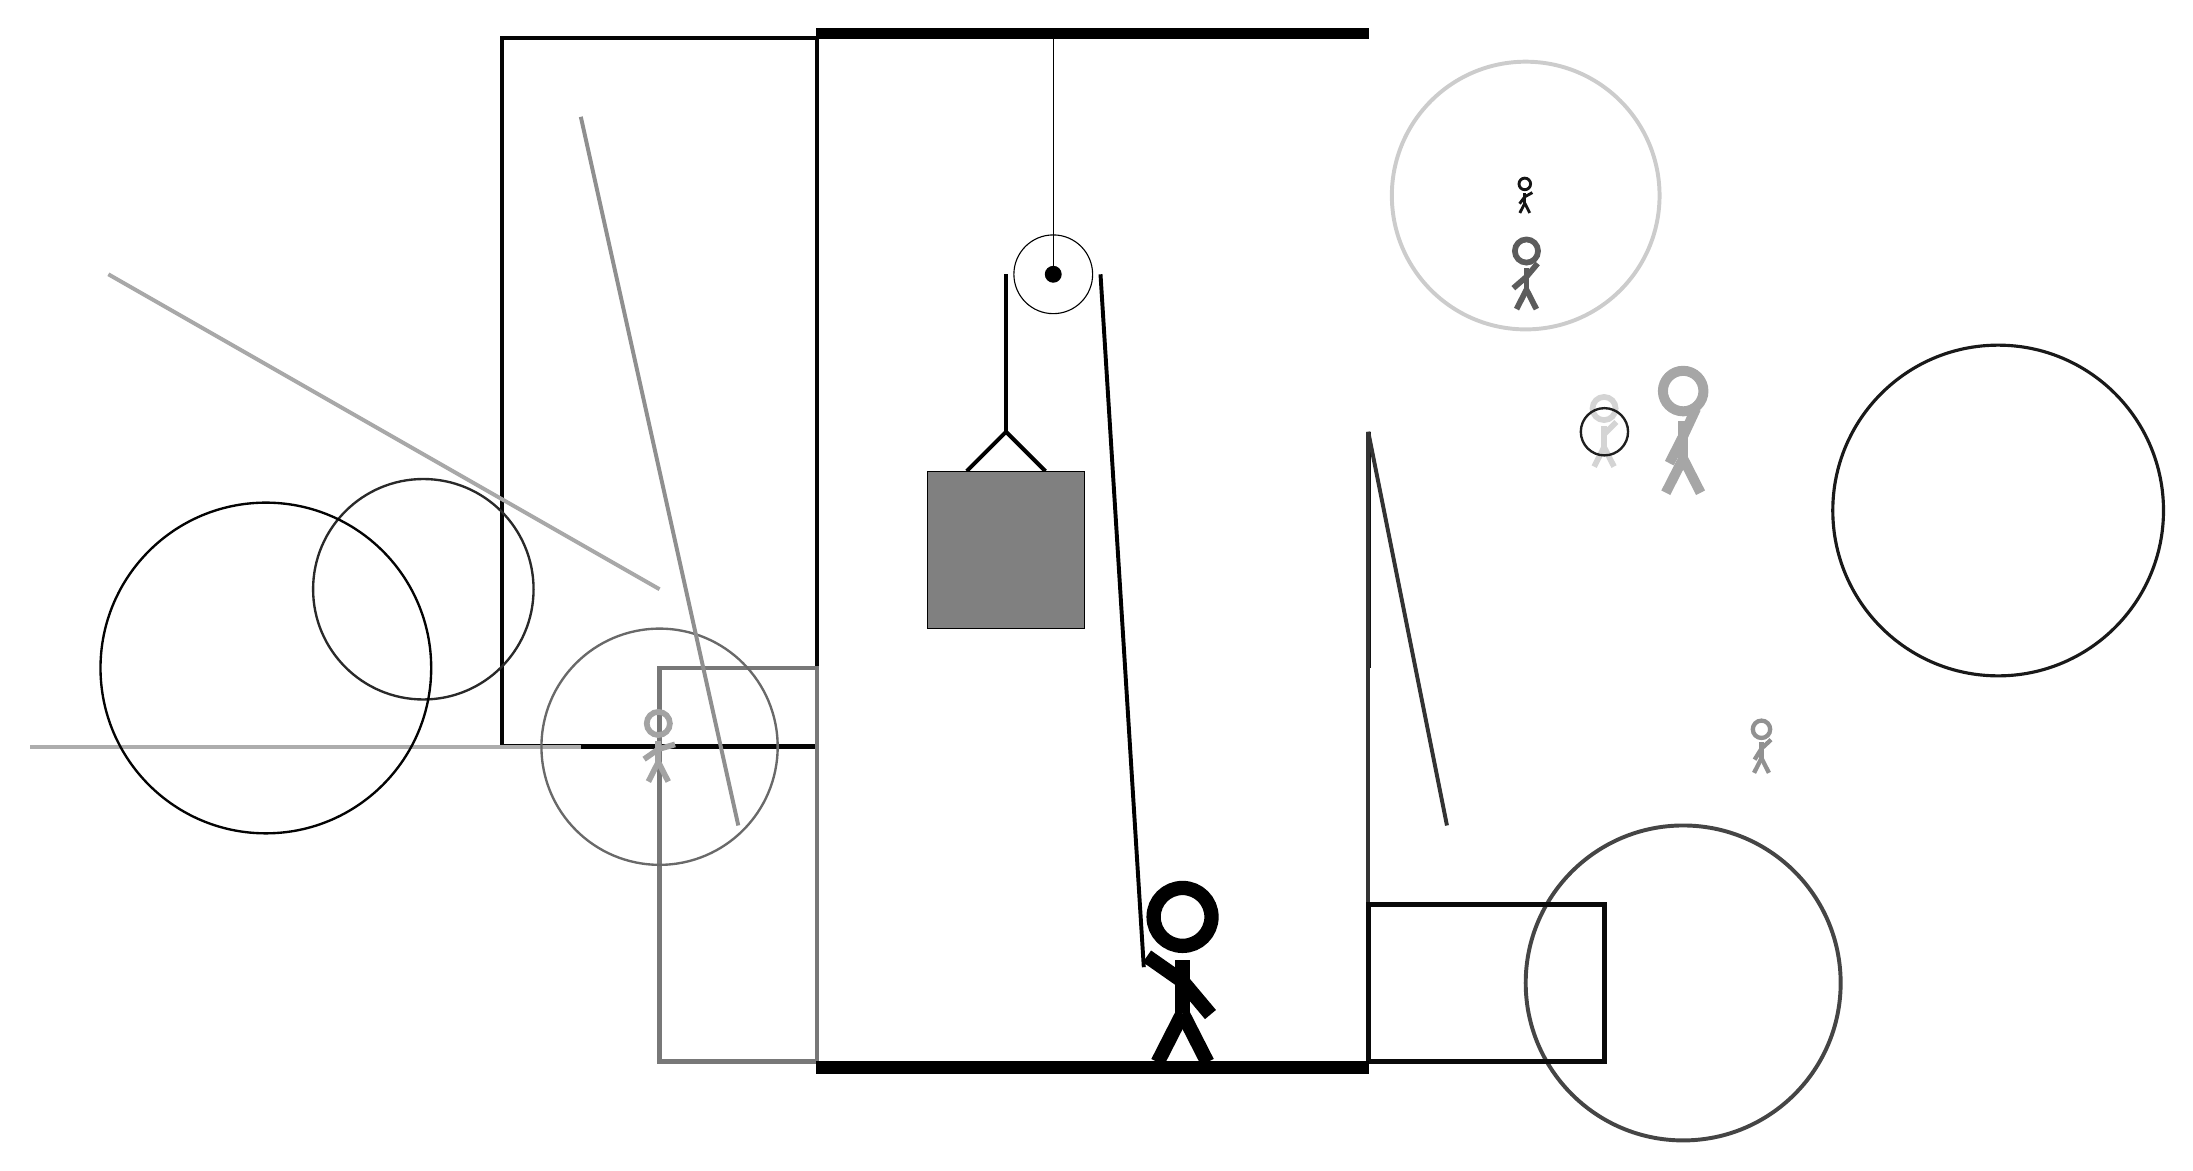
\begin{tikzpicture}
		%%%%% START %%%%%
		
		\draw[fill=black] (-2, 10) rectangle (5, 10.125);
		
		\draw (1, 7) circle (0.5);
		\draw[fill=black] (1, 7) circle (0.1);
		\draw (1, 10) -- (1, 7);
		
		\draw[line width=0.5mm] (-0.1, 4.5) -- (0.4, 5.0) -- (0.9, 4.5);
		\draw[fill=black!50] (-0.6, 4.5) rectangle (1.4, 2.5);
		
		\draw[line width=0.5mm] (0.4, 7) -- (0.4, 5.0);
		\centerarc[line width=0.5mm](1, 7)(0:180:0.6);
		\draw[line width=0.5mm](1.6, 7) -- (2.15, -1.8);
		
		\node[line width=0.4mm, color=black!64] at (7, 7) {\Strichmaxerl[4][41][50]};
		
		\draw[line width=0.6mm, color=black!98] (-2, 1) rectangle (-6, 10);
		\draw [line width=0.4mm, color=black!90](13, 4) circle (2.1);
		\node[line width=0.7mm, color=black!92] at (7, 8) {\Strichmaxerl[2][53][29]};
		\draw [line width=0.5mm, color=black!50](-6, 5) circle (0.0);
		
		\draw[line width=0.6mm, color=black!53] (-2, 2) rectangle (-4, -3);
		
		\node[line width=0.2mm, color=black!43] at (10, 1) {\Strichmaxerl[3][58][43]};
		\node[line width=0.7mm, color=black!17] at (8, 5) {\Strichmaxerl[4][89][45]};
		\draw [line width=0.3mm, color=black!20](-5, -1) circle (0.0);
		\draw[line width=0.5mm, color=black!32](-5, 1) -- (-12, 1);
		\node[line width=0.6mm, color=black!36] at (-4, 1) {\Strichmaxerl[4][35][16]};
		\draw[line width=0.6mm, color=black!93] (5, 5) rectangle (5, 2);
		\draw[line width=0.5mm, color=black!80](5, -1) -- (5, 5);
		\draw [line width=0.3mm, color=black!59](-4, 1) circle (1.5);
		\draw[line width=0.5mm, color=black!44](-5, 9) -- (-3, 0);
		\draw [line width=0.5mm, color=black!73](9, -2) circle (2.0);
		
		\draw [line width=0.5mm, color=black!20](7, 8) circle (1.7);
		\draw[line width=0.5mm, color=black!80](6, 0) -- (5, 5);
		\draw [line width=0.3mm, color=black!84](-7, 3) circle (1.4);
		
		\draw [line width=0.3mm, color=black!88](8, 5) circle (0.3);
		\draw[line width=0.6mm, color=black!96] (5, -1) rectangle (8, -3);
		
		\node[line width=0.7mm, color=black!35] at (9, 5) {\Strichmaxerl[7][63][65]};
		\draw[line width=0.5mm, color=black!34](-4, 3) -- (-11, 7);
		\draw [line width=0.3mm, color=black!99](-9, 2) circle (2.1);
		
		\node at (2.6, -1.9) {\Strichmaxerl[10][-35][-50]};
		
		\draw[fill=black] (-2, -3) rectangle (5, -3.15);
		
		%%%%% END %%%%%
	\end{tikzpicture}
\end{document}